% Options for packages loaded elsewhere
\PassOptionsToPackage{unicode}{hyperref}
\PassOptionsToPackage{hyphens}{url}
\PassOptionsToPackage{dvipsnames,svgnames,x11names}{xcolor}
%
\documentclass[
  letterpaper,
  DIV=11,
  numbers=noendperiod]{scrartcl}

\usepackage{amsmath,amssymb}
\usepackage{iftex}
\ifPDFTeX
  \usepackage[T1]{fontenc}
  \usepackage[utf8]{inputenc}
  \usepackage{textcomp} % provide euro and other symbols
\else % if luatex or xetex
  \usepackage{unicode-math}
  \defaultfontfeatures{Scale=MatchLowercase}
  \defaultfontfeatures[\rmfamily]{Ligatures=TeX,Scale=1}
\fi
\usepackage{lmodern}
\ifPDFTeX\else  
    % xetex/luatex font selection
\fi
% Use upquote if available, for straight quotes in verbatim environments
\IfFileExists{upquote.sty}{\usepackage{upquote}}{}
\IfFileExists{microtype.sty}{% use microtype if available
  \usepackage[]{microtype}
  \UseMicrotypeSet[protrusion]{basicmath} % disable protrusion for tt fonts
}{}
\makeatletter
\@ifundefined{KOMAClassName}{% if non-KOMA class
  \IfFileExists{parskip.sty}{%
    \usepackage{parskip}
  }{% else
    \setlength{\parindent}{0pt}
    \setlength{\parskip}{6pt plus 2pt minus 1pt}}
}{% if KOMA class
  \KOMAoptions{parskip=half}}
\makeatother
\usepackage{xcolor}
\setlength{\emergencystretch}{3em} % prevent overfull lines
\setcounter{secnumdepth}{-\maxdimen} % remove section numbering
% Make \paragraph and \subparagraph free-standing
\ifx\paragraph\undefined\else
  \let\oldparagraph\paragraph
  \renewcommand{\paragraph}[1]{\oldparagraph{#1}\mbox{}}
\fi
\ifx\subparagraph\undefined\else
  \let\oldsubparagraph\subparagraph
  \renewcommand{\subparagraph}[1]{\oldsubparagraph{#1}\mbox{}}
\fi


\providecommand{\tightlist}{%
  \setlength{\itemsep}{0pt}\setlength{\parskip}{0pt}}\usepackage{longtable,booktabs,array}
\usepackage{calc} % for calculating minipage widths
% Correct order of tables after \paragraph or \subparagraph
\usepackage{etoolbox}
\makeatletter
\patchcmd\longtable{\par}{\if@noskipsec\mbox{}\fi\par}{}{}
\makeatother
% Allow footnotes in longtable head/foot
\IfFileExists{footnotehyper.sty}{\usepackage{footnotehyper}}{\usepackage{footnote}}
\makesavenoteenv{longtable}
\usepackage{graphicx}
\makeatletter
\def\maxwidth{\ifdim\Gin@nat@width>\linewidth\linewidth\else\Gin@nat@width\fi}
\def\maxheight{\ifdim\Gin@nat@height>\textheight\textheight\else\Gin@nat@height\fi}
\makeatother
% Scale images if necessary, so that they will not overflow the page
% margins by default, and it is still possible to overwrite the defaults
% using explicit options in \includegraphics[width, height, ...]{}
\setkeys{Gin}{width=\maxwidth,height=\maxheight,keepaspectratio}
% Set default figure placement to htbp
\makeatletter
\def\fps@figure{htbp}
\makeatother
% definitions for citeproc citations
\NewDocumentCommand\citeproctext{}{}
\NewDocumentCommand\citeproc{mm}{%
  \begingroup\def\citeproctext{#2}\cite{#1}\endgroup}
\makeatletter
 % allow citations to break across lines
 \let\@cite@ofmt\@firstofone
 % avoid brackets around text for \cite:
 \def\@biblabel#1{}
 \def\@cite#1#2{{#1\if@tempswa , #2\fi}}
\makeatother
\newlength{\cslhangindent}
\setlength{\cslhangindent}{1.5em}
\newlength{\csllabelwidth}
\setlength{\csllabelwidth}{3em}
\newenvironment{CSLReferences}[2] % #1 hanging-indent, #2 entry-spacing
 {\begin{list}{}{%
  \setlength{\itemindent}{0pt}
  \setlength{\leftmargin}{0pt}
  \setlength{\parsep}{0pt}
  % turn on hanging indent if param 1 is 1
  \ifodd #1
   \setlength{\leftmargin}{\cslhangindent}
   \setlength{\itemindent}{-1\cslhangindent}
  \fi
  % set entry spacing
  \setlength{\itemsep}{#2\baselineskip}}}
 {\end{list}}
\usepackage{calc}
\newcommand{\CSLBlock}[1]{\hfill\break\parbox[t]{\linewidth}{\strut\ignorespaces#1\strut}}
\newcommand{\CSLLeftMargin}[1]{\parbox[t]{\csllabelwidth}{\strut#1\strut}}
\newcommand{\CSLRightInline}[1]{\parbox[t]{\linewidth - \csllabelwidth}{\strut#1\strut}}
\newcommand{\CSLIndent}[1]{\hspace{\cslhangindent}#1}

\KOMAoption{captions}{tableheading}
\makeatletter
\@ifpackageloaded{caption}{}{\usepackage{caption}}
\AtBeginDocument{%
\ifdefined\contentsname
  \renewcommand*\contentsname{Table of contents}
\else
  \newcommand\contentsname{Table of contents}
\fi
\ifdefined\listfigurename
  \renewcommand*\listfigurename{List of Figures}
\else
  \newcommand\listfigurename{List of Figures}
\fi
\ifdefined\listtablename
  \renewcommand*\listtablename{List of Tables}
\else
  \newcommand\listtablename{List of Tables}
\fi
\ifdefined\figurename
  \renewcommand*\figurename{Figure}
\else
  \newcommand\figurename{Figure}
\fi
\ifdefined\tablename
  \renewcommand*\tablename{Table}
\else
  \newcommand\tablename{Table}
\fi
}
\@ifpackageloaded{float}{}{\usepackage{float}}
\floatstyle{ruled}
\@ifundefined{c@chapter}{\newfloat{codelisting}{h}{lop}}{\newfloat{codelisting}{h}{lop}[chapter]}
\floatname{codelisting}{Listing}
\newcommand*\listoflistings{\listof{codelisting}{List of Listings}}
\makeatother
\makeatletter
\makeatother
\makeatletter
\@ifpackageloaded{caption}{}{\usepackage{caption}}
\@ifpackageloaded{subcaption}{}{\usepackage{subcaption}}
\makeatother
\ifLuaTeX
  \usepackage{selnolig}  % disable illegal ligatures
\fi
\usepackage{bookmark}

\IfFileExists{xurl.sty}{\usepackage{xurl}}{} % add URL line breaks if available
\urlstyle{same} % disable monospaced font for URLs
\hypersetup{
  pdftitle={DSCI 310: Predicting Wine Cultivars},
  pdfauthor={Zhibek Dzhunusova, Andrea Jackman, Kaylan Wallace \& Chuxuan Zhou},
  colorlinks=true,
  linkcolor={blue},
  filecolor={Maroon},
  citecolor={Blue},
  urlcolor={Blue},
  pdfcreator={LaTeX via pandoc}}

\title{DSCI 310: Predicting Wine Cultivars}
\author{Zhibek Dzhunusova, Andrea Jackman, Kaylan Wallace \& Chuxuan
Zhou}
\date{}

\begin{document}
\maketitle

\renewcommand*\contentsname{Table of contents}
{
\hypersetup{linkcolor=}
\setcounter{tocdepth}{3}
\tableofcontents
}
\subsection{Summary}\label{summary}

In this project, we will predict what cultivar a wine was derived from
based on its chemical properties.

The data was sourced from the UCI Machine Learning Repository (Aeberhard
and Forina 1991). It contains data about various wines from Italy
derived from three different cultivars. Each row represents the chemical
and physical properties of a different wine, such as its concentration
of alcohol, magnesium level and hue.

\subsection{Introduction}\label{introduction}

Wine is a beverage that has been enjoyed by humans for thousands of
years (Fehér, Lengyel, and Lugasi 2007). Consequently, humans have a
long agricultural history with the grape plant which has led to the
development of many different cultivars: grape plants selected and breed
for their desirable characteristics (Harutyunyan and Malfeito-Ferreira
2022). Our dataset contains information about twelve chemical properties
of \(178\) red wines made from three grape cultivars in Italy.

The recorded chemical properties include:

\begin{enumerate}
\def\labelenumi{\arabic{enumi}.}
\tightlist
\item
  Alcohol content
\item
  Malic acid (gives the wine a fruity flavour)
\item
  Ash (left over inorganic matter from the wine-making process)
\item
  Alkalinity of ash (ability to resist acidification)
\item
  Magnesium, total phenols (contribute to bitter flavour of wine)
\item
  Flavanoids (antioxidants that contribute to bitter flavour and aroma
  of wine)
\item
  Nonflavanoid phenols (weakly acidic)
\item
  Proanthocyanins (bitter smell)
\item
  Color intensity
\item
  Hue
\item
  The ratio of OD280 to OD315 of diluted wines (protein concentration)
\item
  Proline (main amino acid in wine, important aspect of the flavour)
  (Bai, Wang, and Li 2019).
\end{enumerate}

Using this dataset, our predictive question is: ``What is the cultivar
of an unknown wine based on the chemical properties?''

Identifying the chemical properties that distinguish cultivars enables
farmers to make informed decisions about grape cultivation, aligning
grape varieties with desired wine characteristics. By selecting
cultivars known for specific flavor profiles or chemical compositions,
farmers can tailor vineyard practices to meet market demands
effectively. Moreover, this knowledge empowers brewers to experiment
with wine compositions, fostering innovation and the creation of novel
flavors. Armed with a deep understanding of wine chemistry, brewers can
also strategically market their products, ensuring effective
communication of the unique qualities and appeal of each wine to
consumers.

\subsection{Exploratory Data Analysis}\label{exploratory-data-analysis}

\begin{table}

\caption{\label{tbl-summarystats}Summary statistics for the raw data.}

\centering{

\begin{verbatim}


|    alcohol| malicacid|      ash| alcalinity_of_ash|
|----------:|---------:|--------:|-----------------:|
| 11.0300000|  0.740000| 1.360000|         10.600000|
| 14.8300000|  5.800000| 3.230000|         30.000000|
| 13.0006180|  2.336348| 2.366517|         19.494944|
|  0.8118265|  1.117146| 0.274344|          3.339564|




| magnesium| total_phenols| flavanoids| nonflavanoid_phenols|
|---------:|-------------:|----------:|--------------------:|
|  70.00000|      0.980000|  0.3400000|            0.1300000|
| 162.00000|      3.880000|  5.0800000|            0.6600000|
|  99.74157|      2.295112|  2.0292697|            0.3618539|
|  14.28248|      0.625851|  0.9988587|            0.1244533|




| proanthocyanins| color_intensity|       hue| X0D280_0D315_ratio|
|---------------:|---------------:|---------:|------------------:|
|       0.4100000|        1.280000| 0.4800000|          1.2700000|
|       3.5800000|       13.000000| 1.7100000|          4.0000000|
|       1.5908989|        5.058090| 0.9574494|          2.6116854|
|       0.5723589|        2.318286| 0.2285716|          0.7099904|




|   proline|
|---------:|
|  278.0000|
| 1680.0000|
|  746.8933|
|  314.9075|
\end{verbatim}

}

\end{table}%

In Table~\ref{tbl-summarystats}, we have summarized the mean, maximum,
minimum and standard deviation for all predictors. This gives us a
better idea of the normal range of values for each predictor within our
model.

\begin{figure}

\centering{

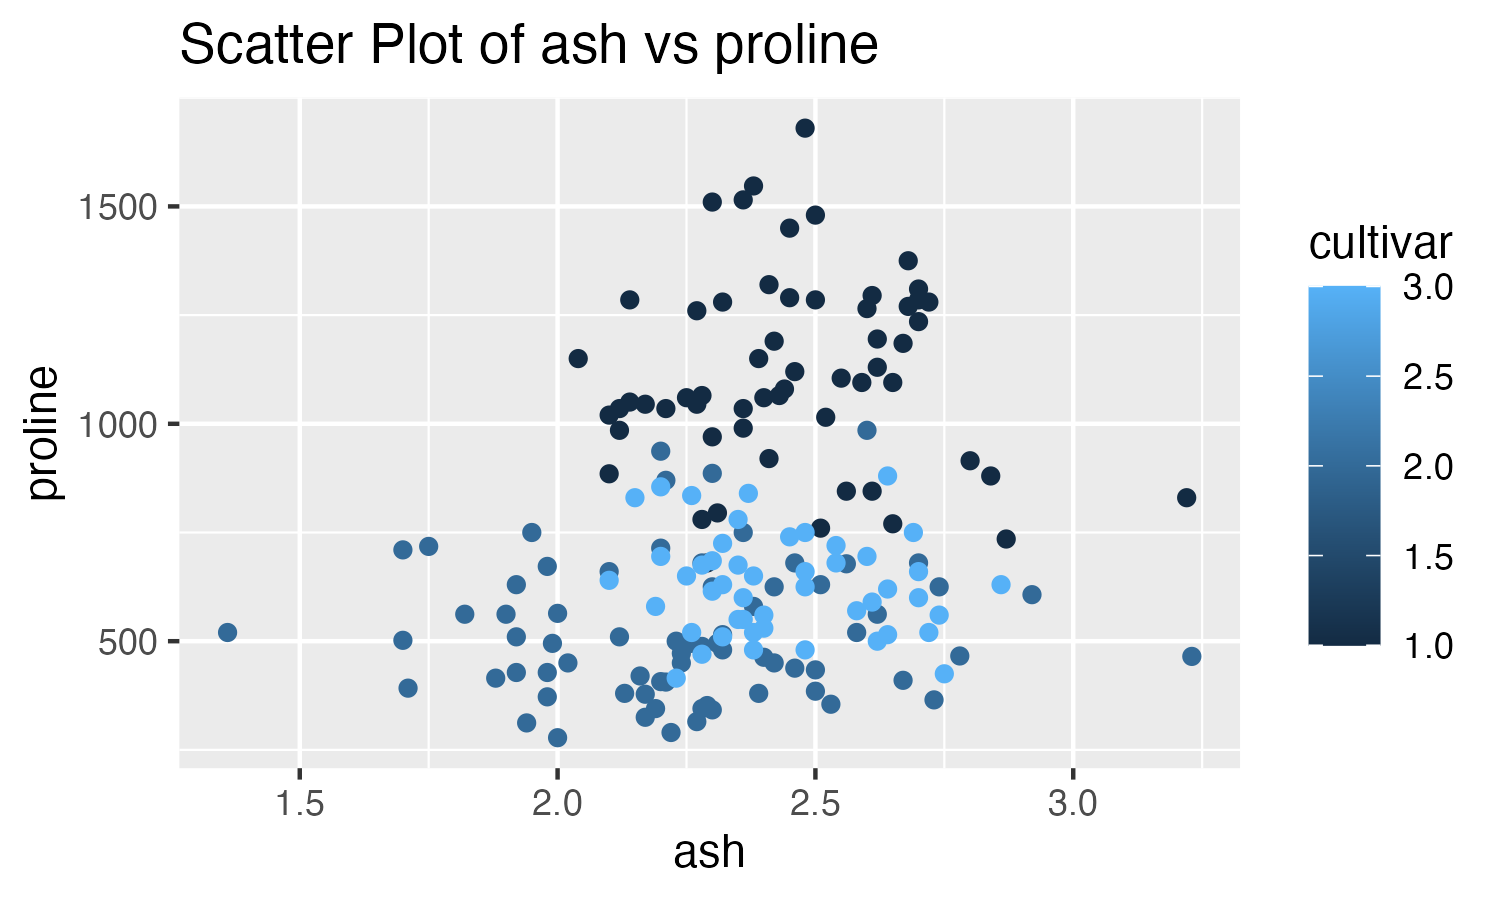
\includegraphics[width=0.9\textwidth,height=\textheight]{../results/scatterplot.png}

}

\caption{\label{fig-scatterplot}Scatterplot of proline and ash values
for each cultivar}

\end{figure}%

Figure~\ref{fig-scatterplot} depicts the distribution of proline and ash
values for each cultivar. Cultivar 1 has more distinct proline and ash
values while Cultivar 2 and Cultivar 3 overlap more substantially.

\begin{figure}

\centering{

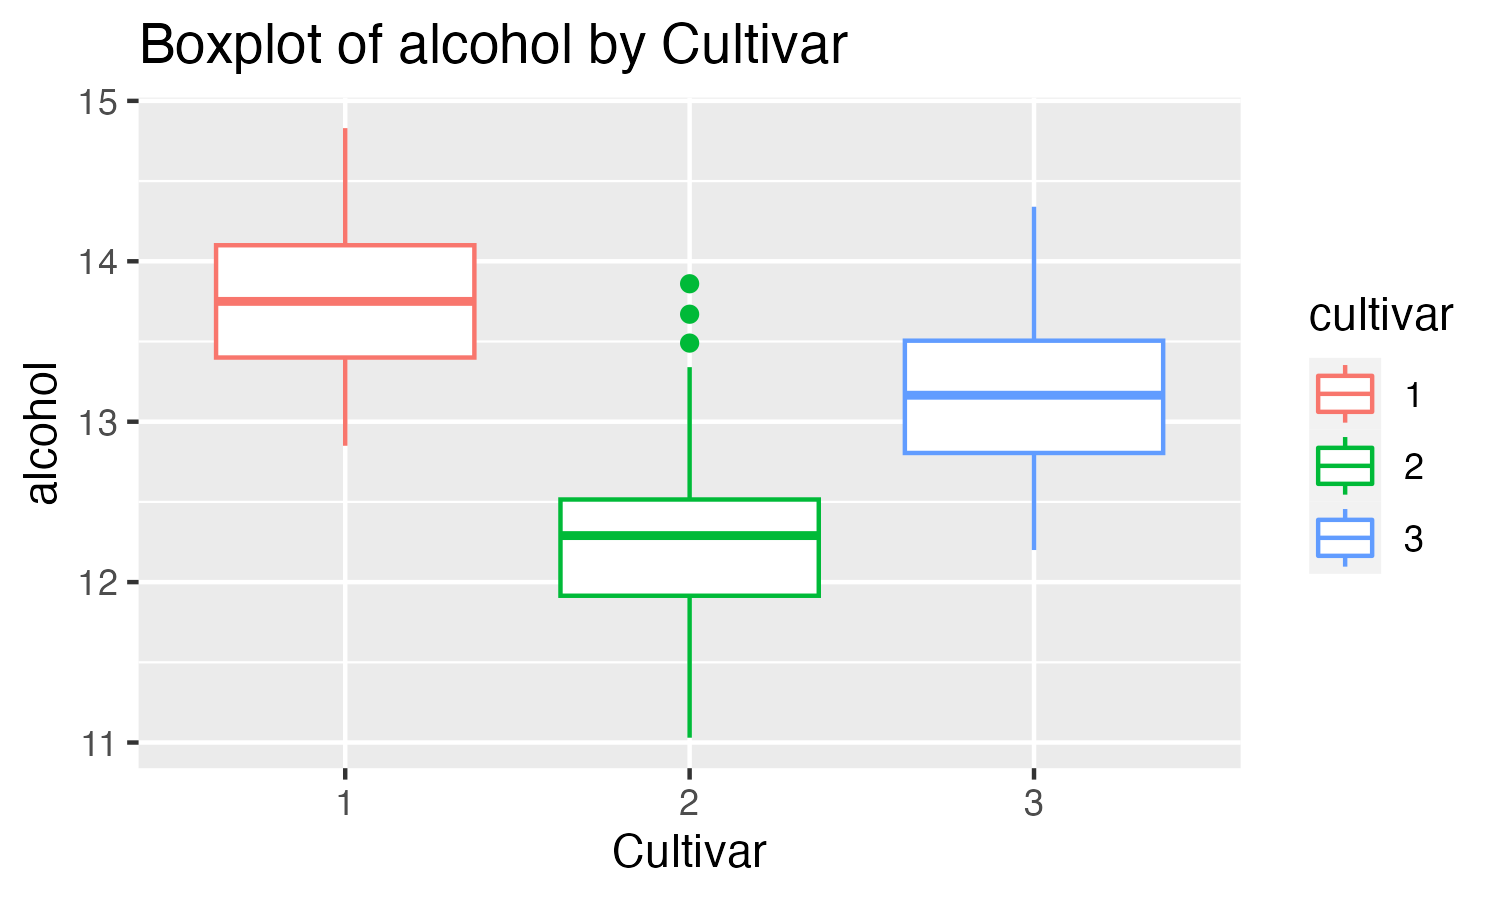
\includegraphics[width=0.9\textwidth,height=\textheight]{../results/boxplot.png}

}

\caption{\label{fig-boxplot}Boxplotplot of alcohol content for each
cultivar}

\end{figure}%

Figure~\ref{fig-boxplot} shows distribution of alcohol content for the
wines from each cultivar. We can see that each cultivar has a narrow
range of values that wines tend to fall within which is relatively
distinct for each cultivar. This means this could be an effective
predictor of cultivar.

\subsection{Methods \& Results}\label{methods-results}

This project utilized a K-nearest neighbours algorithm to predict what
cultivar a wine was derived from based on its various chemical
properties. First, we read in data from the UCI Machine Learning
Repository. It contains data about various wines from Italy derived from
three different cultivars. Each row represents the chemical and physical
properties of a different wine, such as its concentration of alcohol,
magnesium level and hue.

We then tidied the data and balanced the classes of the classification
variable we are interested in. This is because the data set is not
extensively large, so ensuring each class has an equal number of
observations prevents our model from being biased towards a specific
dominant class. Next we calculated some summary statistics to facilitate
exploratory data analysis, with the goal of finding key input variables
for our model.

The data was split into \(75%
\) for the training set and \(25%
\) for the test set. To fine tune our model, we used 5 fold cross
validation, grid search, and graphical methods to choose the optimal
value of \(K\). The result was \(K = 8\) being used in the k-nn model.

\subsection{Discussion}\label{discussion}

\begin{figure}

\centering{


\includegraphics[width=0.9\textwidth,height=\textheight]{../results/accuracy_plot.png}

}

\caption{\label{fig-accuracy-plot}Model accuracy as a function of number
of neighbors}

\end{figure}%

We can see from Figure~\ref{fig-accuracy-plot} that accuracy remains
high across from k = 1 to k = 20. It peaks at around \(0.98 %
\) for \(K = 8\) before decreasing and subsequently increasing back to
\(0.98 %
\) from \(K = 17\) to \(K = 19\). This is a high accuracy value and will
increase the power of our predictive model.

\begin{longtable}[]{@{}rrr@{}}

\caption{\label{tbl-metrics}Model Evaluation metrics.}

\tabularnewline

\toprule\noalign{}
Prediction & Truth & n \\
\midrule\noalign{}
\endhead
\bottomrule\noalign{}
\endlastfoot
1 & 1 & 15 \\
2 & 1 & 0 \\
3 & 1 & 0 \\
1 & 2 & 1 \\
2 & 2 & 17 \\
3 & 2 & 0 \\
1 & 3 & 0 \\
2 & 3 & 0 \\
3 & 3 & 12 \\

\end{longtable}

Table~\ref{tbl-metrics} shows how well our model is able to predict the
cultivar type from predictor variables. We see that it accurately
predicts cultivar for \(44\) of \(45\) data points and only mistakes
cultivar 1 for cultivar 2 once. Therefore, our model has a very high
success rate and will be able to accurately predict the cultivar in most
cases.

Our multiclass k-nn model performed relatively well on the test data,
achieving an accuracy estimate of approximately \(0.98 %
\). The confusion matrix reveals insights into the model's performance
across the three cultivar classes. Notably, while the model demonstrated
strong precision and recall for predicting cultivar 3, it encountered
challenges in accurately classifying cultivar 2. This aligns with our
initial hypothesis that certain chemical properties may serve as
distinguishing factors for wine cultivars.

However, despite the model's overall success, its limitations in
predicting cultivar 2 suggest avenues for improvement. Future iterations
of the model could benefit from refining input variables to better
capture the nuances of each cultivar's chemical composition. Moreover,
our findings underscore the importance of further investigation into the
unique characteristics of cultivar 3, which consistently stood out in
our predictions.

By elucidating the chemical properties that differentiate wine
cultivars, our study contributes to the broader goal of simplifying wine
classification for consumers. Ultimately, this research not only
enhances our understanding of wine chemistry but also has practical
implications for wine enthusiasts and industry professionals alike.

\subsection*{References}\label{references}
\addcontentsline{toc}{subsection}{References}

\phantomsection\label{refs}
\begin{CSLReferences}{1}{0}
\bibitem[\citeproctext]{ref-data-source}
Aeberhard, Stefan, and M. Forina. 1991. {``Wine.''}
\url{https://doi.org/10.24432/C5PC7J}.
\url{https://doi.org/10.24432/C5PC7J}.

\bibitem[\citeproctext]{ref-id-categories}
Bai, X., L. Wang, and H. Li. 2019. {``Identification of Red Wine
Categories Based on Physicochemical Properties.''} In
\emph{International Conference on Educational Technology, Management,
and Humanities Science}, 1443--48.
\url{https://doi.org/10.25236/etmhs.2019.309}.

\bibitem[\citeproctext]{ref-cultural-history}
Fehér, J., G. Lengyel, and A. Lugasi. 2007. {``The Cultural History of
Wine---Theoretical Background to Wine Therapy.''} \emph{Central European
Journal of Medicine} 2 (4): 379--91.
\url{https://doi.org/10.2478/s11536-007-0048-9}.

\bibitem[\citeproctext]{ref-rise-of-wine}
Harutyunyan, M., and M. Malfeito-Ferreira. 2022. {``The Rise of Wine
Among Ancient Civilizations Across the Mediterranean Basin.''}
\emph{Heritage} 5 (2): Article 2.
\url{https://doi.org/10.3390/heritage5020043}.

\end{CSLReferences}



\end{document}
